\documentclass[class=article, crop=false]{standalone}
\usepackage[subpreambles=true]{standalone}
\usepackage{import}
\usepackage[utf8]{inputenc}
\usepackage[table]{xcolor}
\usepackage{tikz}
\usepackage{hyperref}
\usepackage{amsmath}
\usepackage{listings}
\usepackage{pdflscape}
\usepackage{booktabs}
\usepackage{cleveref}

\usepackage[margin=1in]{geometry}

\ifstandalone
\usepackage{color}
\usepackage{xcolor}
\usepackage{caption}
\usepackage{courier}

\lstdefinelanguage{efflang}
{
    % list of keywords
    morekeywords={
        let,
        perform,
        continue,
        val,
        effect,
        in,
        if, then, else,
        with, handle, handler,
        finally,
        match,
        exception,
        of
    },
    sensitive=false,
    morecomment=[s]{(*}{*)},
    morestring=[b]"
}

\lstdefinelanguage{scheme}
{
    % list of keywords
    morekeywords={
        define, call/cc, lambda
    },
    sensitive=false,
    morecomment=[s]{\#|}{|\#},
    morestring=[b]"
}

\lstset{
  basicstyle=\small\ttfamily, % Default font
  numberstyle=\small,          % Style of line numbers
  numbersep=5pt,              % Margin between line numbers and text
  tabsize=2,                  % Size of tabs
  extendedchars=true,
  breaklines=true,            % Lines will be wrapped
  keywordstyle=\color{red},
  frame=b,
  numbers=left,
  numberstyle=\footnotesize\color{gray},
  numbersep=10pt,
  captionpos=t,
  stringstyle=\color{purple!80!blue}\ttfamily, % Color of strings
  showspaces=false,
  showtabs=false,
  xleftmargin=17pt,
  framexleftmargin=17pt,
  framexbottommargin=4pt,
  showstringspaces=false
}

\DeclareCaptionFont{white}{\color{white}}
\DeclareCaptionFormat{listing}{\colorbox[cmyk]{0.43, 0.35, 0.35,0.01}{\parbox{\textwidth}{\hspace{15pt}#1#2#3}}}
\captionsetup[lstlisting]{format=listing,labelfont=white,textfont=white, singlelinecheck=false, margin=0pt, font={bf,footnotesize}}

\newcommand{\mylisting}[4]{%
\noindent
\begin{minipage}{\textwidth}
\lstinputlisting[
  language=#1,
  caption={#2},
  label=#3
  ]{#4}
\end{minipage}
  }

\lstset{language=efflang}
\fi

\ifstandalone
\usepackage{stmaryrd}
\usepackage{framed}

\renewcommand{\leadsto}{\rightsquigarrow}
\providecommand{\dmid}{\ \parallel \ }

\providecommand{\effFalse}{\mathbf{false}}
\providecommand{\effTrue}{\mathbf{true}}
\providecommand{\effLeft}{\mathbf{Left}\ }
\providecommand{\effRight}{\mathbf{Right\ }}
\providecommand{\effFun}{\mathbf{fun}\ }
\providecommand{\effRecFun}{\mathbf{recfun}\ }
\providecommand{\effHandler}{\mathbf{handler}\ }
\providecommand{\effVal}{\mathbf{val}\ }
\providecommand{\effWith}{\mathbf{with}\ }
\providecommand{\effHandle}{\ \mathbf{handle}\ }
\providecommand{\effIf}{\mathbf{if}\ }
\providecommand{\effThen}{\ \mathbf{then}\ }
\providecommand{\effElse}{\ \mathbf{else}\ }
\providecommand{\effAbsurd}{\mathbf{absurd}\ }
\providecommand{\effMatch}{\mathbf{match}\ }
\providecommand{\effLet}{\mathbf{let}\ }
\providecommand{\effIn}{\ \mathbf{in}\ }
\providecommand{\effRec}{\mathbf{rec}\ }
\providecommand{\effEffect}{\mathbf{effect}\ }
\providecommand{\effFinally}{\mathbf{finally}\ }
\providecommand{\effOp}{\mathtt{op}}
\providecommand{\effPerform}{\mathbf{perform}\ }
\providecommand{\tto}{\twoheadrightarrow}

\providecommand{\handlerType}{\Rightarrow}
\providecommand{\boolType}{\mathtt{bool}}
\providecommand{\unitType}{\mathtt{unit}}
\providecommand{\emptyType}{\mathtt{empty}}

\providecommand{\defEq}{\stackrel{\text{def}}{=}}

\providecommand{\cek}[1]{\langle #1 \rangle}
\providecommand{\secd}[1]{\langle #1 \rangle}
\providecommand{\shade}[1]{\langle #1 \rangle}

\providecommand{\irId}{\mathbf{Id}}
\providecommand{\irConst}{\mathbf{Const}}
\providecommand{\irBox}{\mathbf{Box}}
\providecommand{\irFun}{\mathbf{Fun}}
\providecommand{\irHandler}{\mathbf{Handler}}
\providecommand{\irVal}{\mathbf{Return}}
\providecommand{\irIf}{\mathbf{If}}
\providecommand{\irLetIn}{\mathbf{LetIn}}
\providecommand{\irLetRecIn}{\mathbf{LetRecIn}}
\providecommand{\irTopLet}{\mathbf{TopLet}}
\providecommand{\irTopLetRec}{\mathbf{TopLetRec}}
\providecommand{\irPerform}{\mathbf{Perform}}
\providecommand{\irWithHandle}{\mathbf{WithHandle}}
\providecommand{\irBinOp}{\mathbf{BinOp}}
\providecommand{\irFunApp}{\mathbf{FunApp}}
\providecommand{\irGetField}{\mathbf{GetField}}
\providecommand{\irListHead}{\mathbf{ListHead}}
\providecommand{\irListTail}{\mathbf{ListTail}}

\providecommand{\interp}[1]{\llbracket #1 \rrbracket}

\providecommand{\shUnit}{\mathbf{()}}
\providecommand{\shHalt}{\mathbf{halt}}
\providecommand{\shCast}{\mathbf{cast}}
\providecommand{\shRett}{\mathbf{ret2}}
\providecommand{\shApply}{\mathbf{apply}}
\providecommand{\shCastShadow}{\mathbf{castshadow}}
\providecommand{\shKillShadow}{\mathbf{killshadow}}
\providecommand{\shFin}{\mathbf{fin}}
\providecommand{\shThrow}{\mathbf{throw}}

\providecommand{\vmPush}{\textbf{push}}
\providecommand{\vmPop}{\textbf{pop}}
\providecommand{\vmAcc}[1]{\textbf{acc} #1}
\providecommand{\vmConst}[1]{\textbf{const} #1}
\providecommand{\vmHalt}{\textbf{halt}}
\providecommand{\vmJump}[1]{\textbf{jump }#1}
\providecommand{\vmLabel}{\textbf{label}}
\providecommand{\vmBranchIfNot}[1]{\textbf{branchifnot }#1}
\providecommand{\vmApply}{\textbf{apply}}
\providecommand{\vmRet}{\textbf{ret}}
\providecommand{\vmRett}{\textbf{ret2}}
\providecommand{\vmMakeBox}[2]{\textbf{makebox }#1, #2}
\providecommand{\vmGetField}[1]{\textbf{getfield }#1}
\providecommand{\vmListHead}{\textbf{listhead}}
\providecommand{\vmListTail}{\textbf{listtail}}
\providecommand{\vmMakeClosure}[2]{\textbf{makeclosure }#1, #2}
\providecommand{\vmMakeHlosure}[4]{\textbf{makehlosure }#1, #2, #3, #4}
\providecommand{\vmThrow}{\textbf{throw}}
\providecommand{\vmFin}{\textbf{fin}}
\providecommand{\vmCastShadow}{\textbf{castshadow}}
\providecommand{\vmKillShadow}{\textbf{killshadow}}

\providecommand{\hlosure}{\mathcal{H}}
\providecommand{\konts}{\mathcal{C}}

\newenvironment{myfigure}[4][0.75]{
    \def\mywidth{#1}
    \def\mycaption{#3}
    \def\mylabel{#4}
    \definecolor{shadecolor}{rgb}{0.95,0.95,0.95}

    \begin{figure}[#2]
    \centering
    \begin{minipage}{\mywidth\textwidth}
    \begin{shaded*}
}{
    \caption{\mycaption}
    \label{\mylabel}
    \end{shaded*}
    \end{minipage}
    \end{figure}
}
\fi

\begin{document}

This chapter is concerned with the implementation of a CEK interpreter, the
design of a byte code for Eff (SHADEcode), a virtual machine capable of
interpreting this linearised byte code (SHADE VM) and a compiler to this byte
code.

% TODO: arrows
% TODO: include a Requirements Analysis

The chapter is split into two sections: the first part is concerned with the
theory behind the CEK and SHADE machines while the second part is more
practice-oriented.

\section{A CEK machine for Eff}

My implementation uses a CEK interpreter inspired by Hillerström's
machine for Links \cite{hillerstrom2016compilation}.

\subsection{Hlosures}

I talked a lot about closures in the Preparation chapter but the concepts
discussed there did not involve any handlers. In functional languages closures
are used to make it possible to handle functions as values. This non-trivial
because functions can have free variables with values 
dependent on the context. In Eff, handlers are similar in this respect
as they too can have free variables.

\mylisting{efflang}
{A handler parameterised by a free variable $n$}
{lst:parameterised handlers}
{../code_examples/hlosures.eff}

In \autoref{lst:parameterised handlers} the \lstinline|make_handler| function
returns a handler \emph{parameterised} by \lstinline|n|. We see that we need to
remember the value of \verb|n| at the time of the creation of each handler
at runtime. This can be done by attaching the environment $E$ to a handler $H$,
similarly to how one would do this with closures and functions.

In the rest of this chapter I will refer to such structures as \emph{hlosures}
(handler closures) and will denote the hlosure of handler $H$ in the context of
environment $E$ as $\mathcal{H}(H, E)$.

\subsection{Hlosure frames}

When an effect is raised in an Eff program, control is given to a matching
effect case. Now the current delimited continuation must be determined as it
might be used in the body of an effect case. The continuation is delimited by
the with-handle block the \emph{matching handler} is handling. In the
Preparation chapter we saw that we had access to the current continuation at
all times in a CEK machine, however, now we also need to decide which closures
belong to which with-handle blocks in the $K$ stack.

At runtime we always know about the current handler, so we could simply tag all
closures in the $K$ stack with the current handler at the time of its creation.
However, it is a much better idea to simply have a separate $K$ stack per
handler, because that will make the \emph{unwind} operation on the $K$ component
much more efficient (we will unwind handlers and not continuations one by one).

\mylisting{caml}
{The structure of a CEK machine for Eff}
{lst:cek-structure-types}
{../code_examples/cek_structure.ml}

I will call such a structure a \emph{hlosure frame}. Hlosure frames will be the
new entries in the $K$ stack of the CEK machine. They consist of a hlosure and
a \emph{continuation stack} as can be seen in
\autoref{lst:parameterised handlers}.

%  LINE NUMBERS

\subsection{CEK abstract machine}

Now that we know how we account for handlers and delimited continuations in the
CEK machine we can turn our attention to the transition rules of a CEK machine
interpreting Eff (\autoref{fig:cek-machine}).

\subsubsection{Notation}

As expressions do not admit reduction we can simply interpret them in the
context of an environment $\gamma$. For an expression $e$ this is written
$\interp{e}\gamma$ and the notation means that if $e$ is a variable then its
value is looked up from $\gamma$. The runtime representation of functions
$\effFun x \to c$ happens with closures and they are written as tuples of the
form $(x.c, \gamma)$. Hlosures are written as $\mathcal{H}(h, \gamma)$ and the
runtime representation of recursive functions $\effRec f\ x = c$ happens with
recursive closures $\mathcal{R}(f, x.c, \gamma)$ which differ from normal
closures in that they also include the name of the function represented.
The continuation stack in hlosure frames is written as $\mathcal{C}$.

\subsubsection{Function and continuation application}

As we discussed in the Preparation chapter delimited continuations and functions
behave very similarly and there was no need to distinguish them in the abstract
syntax of Eff. However, the runtime system must be aware of what is applied to
an argument! Fortunately, we can always distinguish closures, recursive closures
and continuations at runtime.

Function application or applying closures is standard. When we apply a recursive
closure $\mathcal{R}(f, x.c, \gamma)$ we make sure that we bind $f$ to
$\mathcal{R}(f, x.c, \gamma)$, so that $f$ can be recursively invoked in its
function body. With the hlosure frame representation of $K$, applying a
continuation $\kappa$ is just the same as prepending it to $K$. I would like to
raise attention to how \emph{convenient} this representation is. When an effect
behaves like an exception (i.e., when $\kappa$ is not resumed) all the handlers
up to the handler handling the exception are all in $\kappa$ and are not in $K$
anymore. However, when we do resume $\kappa$ then all the handlers are put back
in place again in $K$, thereby restoring the original execution context the
effect was raised from. This means that there is no extra effort needed to
manage the handler stack separately: the handler stack is managed
\emph{automagically} by the use of continuations.

\begin{myfigure}[0.9]{A CEK machine interpreting Eff}{fig:cek-machine}
    Initialisation:
    $$ c \longrightarrow \cek{c, \{\}, []} $$
    %
    Termination:
    $$ \cek{ \effVal e, \gamma, [] } \longrightarrow \text{halt with } \interp{e}\gamma$$
    Closures, hlosures and resumption from the continuation stack:
    $$ \cek{ \effVal h, \gamma, K} \longrightarrow \cek{\effVal \hlosure(h, \gamma), \gamma, K} $$
    $$ \cek{ \effVal (\effFun x \to c), \gamma, K} \longrightarrow \cek{\effVal (x.c, \gamma), \gamma, K } $$
    $$ \cek{ \effVal e, \gamma, ((x.c, \gamma') :: \mathcal{C}, \mathcal{H}) :: K } \longrightarrow
        \cek{c, \gamma'[x \mapsto \interp{e}\gamma], (\konts, \hlosure) :: K} $$
    %
    Function and continuation application:
    $$ \cek{ (\effFun x \to c)\ e, \gamma, K} \longrightarrow \cek{c, \gamma[x \mapsto \interp{e}\gamma], K } $$
    $$ \cek{ (\mathcal{R}(f, x.c, \gamma')\ v, \gamma, K} \longrightarrow \cek{c, \gamma'[x \mapsto v, f \mapsto \mathcal{R}(f, x.c, \gamma')], K } $$
    $$ \cek{\kappa\ e, \gamma, K } \longrightarrow \cek{ \interp{e} \gamma, \gamma, \kappa\ @\ K } $$
    %
    Perform and with-handle:
    $$ \cek{ \effPerform E(e,k), \gamma, K } \longrightarrow \cek{ \effPerform E(e,k), \gamma, K, [] }_{\text{unwind}} $$
    $$ \cek{ \textbf{with } \hlosure \textbf{ handle } c, \gamma, K } \longrightarrow \cek{ c, \gamma, ([], \hlosure) :: K } $$
    %
    Other standard rules:
    $$ \cek{ \textbf{let } x \leftarrow c_1 \textbf{ in } c_2, \gamma, (\konts, \hlosure) :: K} \longrightarrow 
    \cek{ c_1, \gamma, ((x. c_2, \gamma) :: \konts, \hlosure) :: K } $$
    $$ \cek{\effLet \effRec f\ x = c_1 \effIn c_2, \gamma, K} \longrightarrow
    \cek{c_2, \gamma[f \mapsto \mathcal{R}(f, x.c_1, \gamma)], K} $$
    \begin{align*}
    \cek{ \textbf{if } e \textbf{ then } c_1 \textbf{ else } c_2, \gamma, K } \longrightarrow \cek{ c, \gamma, K } \\
    \text{ where $c = c_1$ if $\interp{e} \gamma = \textbf{true}$; and $c = c_2$ otherwise}
    \end{align*}
\end{myfigure}

\subsubsection{Perform and with-handle}

The remaining two features of Eff can be conveniently implemented with hlosure
frames too. The rule for with-handle blocks simply prepends $([], \mathcal{H})$
to $K$, where $[]$ is an empty continuation stack and $\mathcal{H}$ is a
hlosure representing the handler from the with-handle block.

Performing effects is a little bit more difficult due to the unwinding of the
$K$ component. When an effect is performed we must search for the closest
handler capable of handling the effect. However, we must also concatenate
together all the delimited continuations from the hlosure frames we jump
through. \autoref{fig:cek-k-unwind} depicts concisely how this can be done. The
CEK state is temporarily extended with a fourth component which behaves as an
accumulator for hlosure frames (and hence as an accumulator for delimited
continuations).

If a handler frame contains a hlosure $\mathcal{H}$ that can handle the
performed effect then $\kappa$ (the list of hlosure frames carrying the
delimited continuation in the fourth component) is bound to $k$ and the
identifier of the effect argument from the effect case is bound to $e$ in
$\mathcal{H}'s$ (!) environment. Otherwise, the current hlosure frame is
removed from the CEK state and is appended to $\kappa$ and the unwinding
continues.

\begin{myfigure}[.95]{Unwinding of the K component in the CEK machine}{fig:cek-k-unwind}
    \begin{align*}
        \cek{ \effPerform E(e,k), \gamma, (\konts, \hlosure) :: K, \kappa}_\text{unwind} \longrightarrow
        \cek{ \effPerform E(e,k), \gamma, K, \kappa@[(\konts, \hlosure)] }_\text{unwind} \\
        \text{ if $\hlosure = (H, \_)$ and handler $H$ does not handle effect $E$}
        \end{align*}
        \begin{align*}
        \cek{ \textbf{perform } E(e,k), \gamma, (\konts, \hlosure) :: K, \kappa}_\text{unwind} \longrightarrow
        \cek{ M, \gamma' [x \mapsto (\interp{e}\gamma), k \mapsto \kappa @ [(\konts, \hlosure)]], K} \\
        \text{ if $\hlosure = (H, \gamma')$ and handler $H$ handles effect $E$ with rule $\textbf{effect } E\ x \ k \to M$ }
        \end{align*}
\end{myfigure}

An OCaml code snippet showing how to implement this same functionality can be
found in Appendix \autoref{sec:code-snippets}. A nice feature of functional
languages is that once we get our theory right, the theory usually lends
itself to an almost trivial implementation. This is the case with the CEK
machine too and this is why I will not talk about the implementation in
detail here---however, a typical rule implementation can be found below.
% NOT BELOW

All transition rules are implemented via a \lstinline{step} function which
performs a single step of the transition rules shown in
\autoref{fig:cek-machine}. This can be seen in \autoref{lst:impl-step-func}.

\mylisting{caml}
{A typical implementation of a rule in the \lstinline{step} function}
{lst:impl-step-func}
{../code_examples/step_function.ml}

\section{The SHADE virtual machine}
\label{sec:shade-machine}

The SHADE virtual machine is an SECD-like virtual machine in that it has a dump
component, however, it interprets byte code (SHADEcode, which is described in
\autoref{tab:shade-bytecode}) rather than the source terms of a language. The
name is an anagram from the initials of the main components of the machine: 
\emph{accumulator} (A), \emph{dump} (D), \emph{environment} (E),
\emph{hlosure} (H) and \emph{stack} (S). The rest of this section is concerned
with a description of this machine using its transition rules.
\Cref{sec:shade-illustration} will give an overview of how the byte code
implements the different aspects of the Eff language.

\paragraph{Configuration.}
The state of the machine can be characterised with a two-tuple
$\langle A, D \rangle$ where $A$ is the accumulator and $D$ is a dump. I call
the elements of $D$ \emph{shadows}. Shadows are the SHADE equivalent of CEK
hlosure frames. A shadow is a four-tuple $\langle pc, E, H, S \rangle$, where
$pc$ is the program-counter of the shadow, $E$ is an environment, $H$ is a
hlosure and $S$ is a stack.
\footnote{The SHADE machine had many versions throughout the year and this
final version turns out to be surprisingly similar to the solution Multicore
OCaml uses with its fibres -- the heap-allocated fibres of OCaml show a lot
of resemblance with the shadows of the SHADE machine.}

Only the \emph{top shadow} is executing of all the shadows at any point in the
execution. To avoid having to refer to the top shadow through the $D$ component
I will use the notation $\langle A, d, D \rangle$ instead to denote the SHADE
configuration $\langle A, d :: D \rangle$.

In the program counter field ($pc$) of a shadow I will write the instruction
the program counter points to and its value interchangeably. On the left hand
side of the transition rules it is more convenient to refer to the instruction
and on the right hand side it is often useful to write $pc+1$ to mean that the
program counter is incremented or write $L$ to mean that we perform a jump to
the label $L$.

\subsection{Transition rules and SHADEcode}

\autoref{fig:shade-machine} shows only transition rules for \emph{inter-shadow
instructions}. These are instructions which implement the interactions between
shadows (i.e., they manipulate the D component of the machine and implement the
Eff-specific features like performing effects, applying continuations, entering
and returning from with-handle blocks and handler cases).

\emph{Intra-shadow} instructions are standard stack machine instructions similar
to those of the Caml Virtual Machine \cite{caml-vm}. I will not give formal
transition rules for these here. \autoref{tab:shade-bytecode} includes all
SHADE instructions and explains their purpose in prose.

The SHADE machine is initialised by loading a program compiled to byte code
and initialising $D$ to a list containing an \emph{empty shadow} with the
default handler $H_{def}$. The default handler is responsible for handling
effects which rise to the toplevel
\footnote{Runtime systems can define built-in effects this way. The Evaluation
chapter will show how can one implement a web server in Eff by defining 2
built-in effects which interact with the Linux kernel.}.
The machine terminates when it reaches the \vmHalt\ instruction.

\paragraph{Communication between shadows.}

I will start to introduce the SHADE byte code and the SHADE transition rules.
Unfortunately, there is a circular dependency between the concepts in this
section. I apologise in advance for starting to talk about the compilation
this suddenly, but the cycle must be broken somewhere. Let us consider how
with-handle blocks are compiled:
$$ \interp{\irWithHandle\ (h, e)}_s ^ \gamma = \interp{h}_s ^ \gamma; \vmPush; \text{fvs-to-stack}(e, s, \gamma); \vmMakeClosure{N}{L}; \shCastShadow; \shFin.$$
The handler is first compiled and is pushed to the stack. Then the closure of
the with-handle block's body is constructed and a new shadow corresponding to
this block is created by the \vmCastShadow\ instruction. $L$ is a fresh label
denoting the start of the with-handle block's body. The code for the body of
the with-handle block is generated separately. The \vmFin\ instruction invokes
the finally case after control is returned to this shadow again. When this
happens, the hlosure of $h$ is still on the stack of this shadow and this is
the reason why the \vmCastShadow\ instruction does not consume the hlosure from
the stack. It might not be obvious why we need a separate instruction for
finally cases. The reason is that control can return in many ways: it can come
from a value or effect case via a \vmRett\ instruction. However, when many
continuations are resumed in the same with-handle block (think about the Hello
World example), then only the last \vmRett\ instruction actually leaves the
with-handle block and therefore we cannot make the invocation of finally cases
a feature of the \vmRett\ instruction. This is the responsibility of the same
shadow a with-handle block resides in.

\begin{myfigure}[0.95]
    {SHADE machine transition rules}
    {fig:shade-machine}
        Initialisation:
        $$\text{program} \to \shade{\shUnit, (0, \{\}, H_{def}, []), []}$$
        Termination:
        $$ \shade{v, (\shHalt, E, H, S), D} \to v $$
        Transition rules for Eff-specific instructions:
        $$ \shade{\mathcal{C}(cp, \gamma), (\shCastShadow, E, H, \hlosure :: S), D} \to \shade{A, (cp, \gamma, \hlosure, []), (pc+1, E, H, \hlosure :: S) :: D} $$
        $$ \shade{A, (\shKillShadow, E, \hlosure(h, \gamma), S), D} \to  \shade{A, (L_{\text{valcase}(h)}, \gamma, \hlosure(h, \gamma),S), D} $$
        $$ \shade{A, (\shFin, E, H, \hlosure(h, \gamma) :: S), D} \to \shade{A, (L_{\text{fincase}(h)}, \gamma, (pc, E) :: S), D} $$
        $$ \shade{A, (\shThrow\ id, E, H, S), D} \to \shade{A, (\shThrow\ id, E, H, S), D, []}_\text{unwind}^{id} $$
    
        $$ \shade{A, (\shRett, E, H, S), D} \to \shade{A, D} $$
        $$ \shade{A, (\shApply, E, H, \mathcal{C}(cp, \gamma) :: S), D} \to \shade{A, (cp, \gamma, H, (pc, E) :: S), D} $$
        $$ \shade{A, (\shApply, E, H, \kappa :: S), D} \to \shade{A, \kappa\ @\ ((pc, E, H, S) :: D)} $$
    \end{myfigure}

Another important detail is that three syntacticly similar contstructs are not
compiled the same way: the bodies of functions, with-handle blocks and handler
cases.
The body of with-handle blocks
always ends with a \vmKillShadow\  instruction, value cases and effect cases end
with a \vmRett\ instruction, the bodies of functions and finally cases end with
\vmRet.

The reason why the transition rule of \vmKillShadow\ invokes the value case of
the current handler is because the bodies of with-handle blocks end with
\vmKillShadow\ instructions---\vmKillShadow\ does not actually destroy the
current top shadow; it simply prepares it for the execution of the value case
of a handler by jumping to the corresponding label and putting the environment
of the hlosure in $E$. As value cases end with \vmRett\ instructions and they
always destroy the top shadow, the job is finished by the \vmRett\ of a value
case.

If the behaviour of an effect is exception-like then control might not reach
the end of a with-handle block. This justifies why \vmKillShadow\ cannot be
responsible for actually destroying shadows or for invoking the finally case of
a handler which further justifies the existence of the \vmFin\ instruction.

The \vmFin\ instruction implements the invocation of finally cases as a
function call but it also pops the handler the \vmCastShadow\ instruction left
on the stack. With this, Eff effect handlers are implemented.

\paragraph{Similarities with the CEK machine.}
The \vmApply\ instruction implements function and continuation application the
same way it was done in the CEK machine. The \vmThrow\ instruction is used to
perform an effect. When this happens the dump has to be unwound the same way
the $K$ component of the CEK machines needed to be unwound.

\begin{myfigure}[1]{Dump unwinding in SHADE}{fig:shade-stack-unwind}
    $$ \shade{A, \underbrace{(pc, E, H, S)}_d, D, \kappa }_\text{unwind}^{id} \text{ and } H \uparrow id \to \begin{cases}
        \text{Runtime exception} & \text{if } D = [] \\
    \shade{A, d, D', \kappa @ [d]}_\text{unwind}^{id} & \text{if } D = d' :: D' \end{cases} $$

    $$ \shade{A, (pc, E, \hlosure(h, \gamma), S), D, \kappa}_\text{unwind}^{id} \to
        \shade{A, (L_{\text{effcase}(h, id)}, \gamma[x \mapsto A, k \mapsto \kappa] ), D} \text{ if } h \downarrow id $$
\end{myfigure}

\paragraph{Calling convention}

Another fine but important detail is that the calling convention for functions,
continuations \emph{and} effects must match. At the time of the compilation we
have no idea whether an identifier will stand for a function or a continuation.
One might think that this still leaves us many possibilities, but this actually
completely defines the calling convention in SHADE.

We cannot use the stack to pass function or continuation arguments around
because by resuming a continuation we are also restoring shadows and therefore
we lose the access to the current stack. The same goes for returning values.
Hence we must use the accumulator.

% TODO: split table
\begin{table}
\centering
{\renewcommand{\arraystretch}{1.3}
\rowcolors{2}{gray!17}{white}
\begin{tabular}{p{3.2cm}p{6.5cm}p{4.2cm}}
    \toprule
    Instruction & Description & Action \\
    \midrule
    \vmPush & 
        Push the accumulator to the stack. &
        \verb|S := A :: S| \\
    \vmPop  &
        Remove the top element of the stack. &
        \verb|S := S.tail| \\
    \vmAcc{$n$} &
        Copy the $n^\text{th}$ element (0 indexed) of the stack in the accumulator. &
        \verb|A := S[n]| \\
    \vmConst{$c$} &
        Load the constant $c$ to the accumulator. &
        \verb|A := c| \\
    \vmHalt &
        Halt the SHADE machine with the value in A. &
        terminate with A \\
    \vmJump{$L$} &
        Jump to location L. &
        \verb|pc := adress of L| \\
    \vmBranchIfNot{$L$} & 
        If A = false then jump to location L. Otherwise continue with the next
        instruction. &
        \begin{tabular}[t]{@{}l@{}}
            if \verb|A| then \verb|pc := pc + 1|\\
            else \verb|pc := L| \end{tabular} \\
    \vmApply &
        Apply the top of the stack to the accumulator. &
        see \autoref{fig:shade-machine} \\
    \vmRet &
        Return with the value in A. Restore the old program counter and
        environment from S. &
        see \autoref{fig:shade-machine} \\
    \vmRett & 
        Return from a value or effect case with the value in A. Destroy the top
        shadow and increment the program counter of the new top shadow. &
        see \autoref{fig:shade-machine} \\
    \vmThrow \mathtt{effid} &
        Throw an effect. \texttt{effid} is an integer denoting the type of the
        effect being thrown. The argument to the effect resides in the
        accumulator. &
        see \autoref{fig:shade-machine} \\
    \vmFin &
        Invoke the finally case of the hlosure on the top of the stack as a
        function call using the accumulator as the argument. Pop the hlosure
        from the stack. &
        see \autoref{fig:shade-machine} \\
    \vmCastShadow &
        Cast a new shadow. &
        see \autoref{fig:shade-machine} \\
    \vmKillShadow &
        Kill a shadow. &
        see \autoref{fig:shade-machine} \\
    \vmMakeBox{$t$}{$n$} &
        Create a box with tag $t$ using $A$ and the top $n-1$ elements of S. & \\
    \vmGetField{$n$} &
        Load field $n$ (0 indexed) of a box to A. &
        \verb|A := A[n]|\\
    \vmListHead &
        Load the head of a list to A. &
        \verb|A := A.head| \\
    \vmListTail &
        Load the tail of a list to A. &
        \verb|A := A.tail| \\
    \vmMakeClosure{$L$}{$n$} &
        Form an environment of A and the top $n-1$ elements of S and create a
        closure with this environment of location L. &
        \begin{tabular}[t]{@{}l@{}}
            \verb|E = [A, S[0:N]];| \\
            \verb|S.pop(N-1);| \\
            \verb|A := closure(L, E)|
        \end{tabular} \\
    \begin{tabular}[t]{@{}l@{}}
        \textbf{makehlosure} $N$, $L_v$ \\
        $L_f$, $[\overline{L_{e_i}, \mathtt{effid}]$ 
    \end{tabular} &
        Similar to \vmMakeClosure{$L$}{$N$} but with many locations each
        corresponding to a handler case. Effect cases are represented with
        pairs $(L, \mathtt{effid})$ where $L$ is a code pointer of the effect
        case and \mathtt{effid} is an integer identifier of the type of the
        effect being handled.&
        \begin{tabular}[t]{@{}l@{}}
            \verb|E = [A, S[0:N-1]];| \\
            \verb|S.pop(N-1);| \\
            \verb|A := hlosure(|$L_v$, $L_f$,\\
            \quad\quad\quad\quad\quad $L_{e_1}$\verb|,.., E)|
        \end{tabular} \\
        binary operators \textbf{intadd}, \textbf{floatadd}, etc. &
        Perform a binary operation with A and S.top. &
        \begin{tabular}[t]{@{}l@{}}
            \verb|A := bop(A, S.top())| \\
            \verb|S.pop()|
        \end{tabular} \\
    \bottomrule
\end{tabular}}
\caption{SHADEcode, the instruction set of the SHADE machine}
\label{tab:shade-bytecode}
\end{table}

\paragraph{Compiling to SHADEcode}

Compilation to SHADEcode is standard. We keep track of the size of the stack
$s$ and a compilation environment $\gamma$ which tells us where the free
variables of currently compiled expressions reside (stack or environment).
The equation
$$ \interp{\irLetIn\ (x, e_1, e_2)}_s^\gamma = \interp{e_1}_s^\gamma; \vmPush; \interp{e_2}_{s+1}^{\gamma[x \mapsto s]} $$
describes how one can compile let expressions. The expression $e_1$ is compiled
first which generates the code that leaves the value of $e_1$ in the accumulator.
Then a \vmPush\ instruction saves this on the stack and the expression $e_2$ is
compiled with the knowledge that the size of the stack has increased to $s+1$
and the new compilation environment knows that $x$ resides at position $s$ in
the stack ($\gamma[x \mapsto x]$). A full description of the compilation process
in this style can be found in Appendix \autoref{app:theory}.

\subsection{How does SHADEcode implement Eff?}
\label{sec:shade-illustration}

I gave a formal but dry description of the SHADE machine and its bytecode in
the previous section. The reader might rightfully demand an explanation of why
SHADE makes sense for Eff. In this section I will show how the byte code can
implement the various flow of control algebraic effect handlers allow.

It is clear that when no new shadow is cast (no with-handle is used) then the
SHADE machine is essentially a Zinc \cite{leroy1990zinc} machine with all
effects behaving like exceptions. The next page contains various examples and
should give a good insight into how everything fits together.

\begin{figure}
    \centering
    \scalebox{.75}{
        \subimport{../figures/}{impl-no-perform.tex}
    }
    \caption{No effect is performed.}
    \label{fig:shadecode-no-effect}
\end{figure}

\autoref{fig:shadecode-no-effect} shows what happens when no effect is performed
in a with-handle block. The with-handle block is entered via \vmCastShadow\
(a second shadow is cast and we jump to \lstinline{Lwith}). Next, after the
body of the with-handle block executes fully the \vmKillShadow\ instruction
gives the control to the value case. The \vmRett\ instruction at the end of
the value case destroys the second shadow and returns to the default shadow
while increasing the program counter. Now the \vmFin\ instruction is responsible
for executing the finally case and getting rid of the hlosure from the stack.
The \vmRet\ instruction at the end of the finally case simply returns as if it
was a function call and execution halts as the program counter now points to
\vmHalt.

\begin{figure}
    \centering
    \scalebox{.75}{
        \subimport{../figures/}{impl-exception.tex}
    }
    \caption{An effect is performed but its continuation is not resumed.}
    \label{fig:shadecode-exception}
\end{figure}

\autoref{fig:shadecode-exception} depicts a case when the effect has
exception-like behaviour. This case is different from the previous one in that
the \vmKillShadow\ instruction is never executed. However, the \vmRett\
instruction at the end of the effect case of handler $h$ will still destroy the
shadow and return to the \vmFin\ instruction which is executed before the
machine halts as we would expect. The result of the program is \lstinline|86|.

\autoref{fig:shadecode-one-resume} shows an example where the continuation is
resumed in the effect case (this is actually our beloved Hello World again!).
This case is particularly interesting as effects are performed in the
with-handle block, continuations are resumed, the \vmKillShadow\ instruction is
executed and the \vmRett\ of the value case \emph{returns to an effect case}
which then returns to another effect case and finally the top shadow is
destroyed by the \vmRett\ of an effect case just as we saw in the previous
example. The program returns with the string
\lstinline|"Error: got exception oops!"|.

The red dots next to the \vmApply\ instruction are there to show that the dump
is essentially a separate call stack for continuations and effect cases.
Two separate \vmRett\ instructions return to the same \vmApply\ instruction
but first the effect case handling \lstinline{Print "not to be"} is given
control and only after that effect case is finished can the effect case handling
\lstinline{Print "Try"} resume. This program returns the tuple
\lstinline|("confused!", "Try not to be")|.

\begin{figure}
    \centering
    \scalebox{.75}{
        \subimport{../figures/}{impl-one-resume.tex}
    }
    \caption{An effect is performed and its continuation is resumed.}
    \label{fig:shadecode-one-resume}
\end{figure}
 
\autoref{fig:shadecode-two-resume} shows what happens when we take everything to
the next level and use multi-shot continuations (i.e., we resume the same
continuation more than once). This is a typical non-determinism example where
an effect case resumes a continuation with both \lstinline{true} and
\lstinline{false} to determine all the values the with-handle block can evaluate
to. \footnote{We are expecting the result \lstinline{[5,-5,15,5]} as $(x-y)$
can be $(10-5)$, $(10-15)$, $(20-5)$ or $(20-15)$.}
\autoref{fig:shadecode-two-resume} also outlines the structure of the dump.
The red arrows denote the instructions which increase the size of the dump and
the black arrows are just there to show where we are in the execution.
The blue \vmRett\ instructions are those of the value case's and they are only
invoked ``at depth 4'' in the diagram.

Continuations are highlighted with shades of orange. Because all continuations
are invoked twice these must be cloned which can add a significant copy overhead.
This is one way Eff differs from Multicore OCaml. Multicore OCaml only supports
one-shot continuations and programmers must be aware whether they already used
a continuation or not. In Multicore OCaml the same continuation can only be used
when it was cloned before resuming it for the second time. The programmer must
manually do this with the \lstinline|Obj.copy_continuation| call. If the
programmer forgets about this then the program can crash. As Eff is different
in this respect, the SHADE machine always keeps a clean copy of every
continuation which can be cloned on demand when it is resumed.
This is an inefficiency but is necessary for correctness.

\begin{landscape}
    \begin{figure}
        \centering
        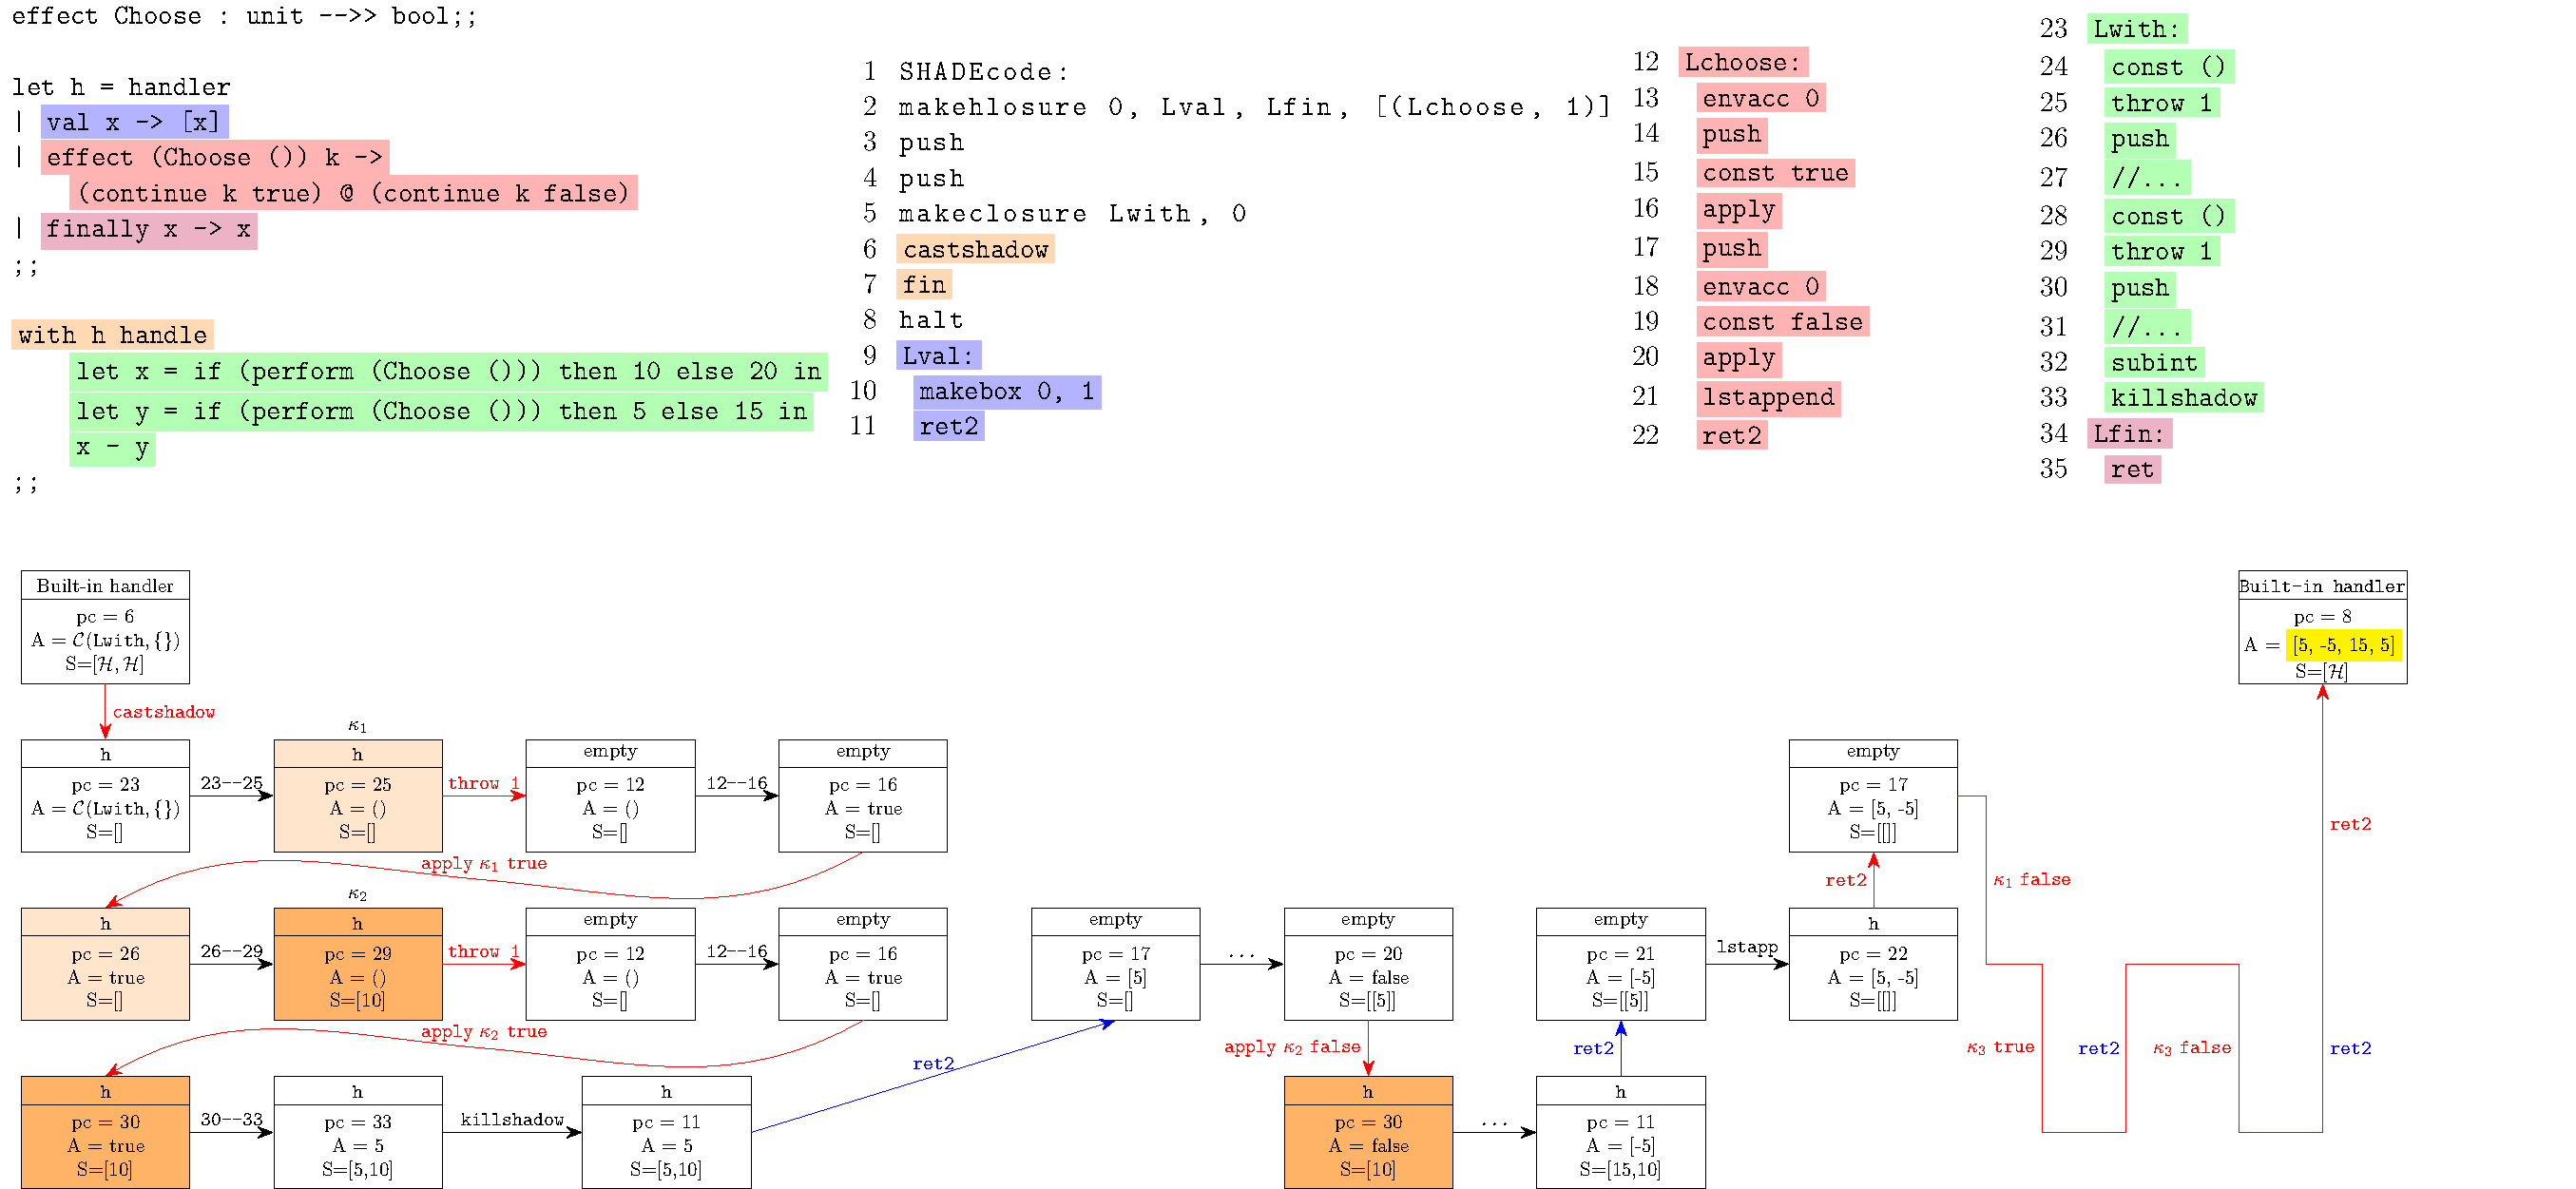
\includegraphics[width=\paperwidth]{../figures/impl-two-resume.pdf}
        \caption{Non-determinism: multi-shot continuations can be resumed more than once in Eff}
        \label{fig:shadecode-two-resume}
    \end{figure}
\end{landscape}

\section{Software engineering}

Now that the theory is sorted out I can present my OCaml implementation of the
project.

\subsection{Repository structure}

The repository of my OCaml implementation is structured as a typical OCaml
package. A \verb|bin| directory contains the entry points of the executables
generated, the \verb|lib| directory contains the collection of modules making
up the project. The \verb|test| directory contains unit tests and regression
tests.

% TODO: coloring on this graph + Tikz it
% TODO: code audit -- complete LoC
\begin{figure}
    \centering
    %\includegraphics[width=\textwidth]{../figures/dependencies.pdf}
    \caption{Dependency graph of the modules in \texttt{lib}}
    \label{fig:dependencies}
\end{figure}

\begin{table}
    \centering
    {\renewcommand{\arraystretch}{1.3}
    \rowcolors{2}{gray!17}{white}
    \begin{tabular}{p{3cm}p{10cm}}
    \toprule
    \textbf{Module name} & \textbf{Purpose} & LoC \\
    \midrule
    \textbf{Stx} & 
        Specifies Eff syntax trees. The \verb|ocamllex| and the Menhir parser
        generator uses this module to generate a parser for Eff. &
        X \\
    \textbf{Preprocess} &
        Implements preprocessing functionalities on ASTs. At this stage all
        identifiers are given unique integer De Bruijn indices
        and some syntactic sugars are removed.  &
        X \\
    \textbf{Translate} &
        Implements various translation functionalities. Erases the distinctions
        between computations and expressions and implements translations from
        ASTs to various intermediate representations. &
        X \\
    \textbf{Cek\_types} & Contains the specification of the CEK machine
        discussed in this chapter. &
        X \\
    \textbf{Cek} &
        Implementation of the CEK machine. &
        X \\
    \textbf{Ir} &
        Specification of an intermediate representation close to \emph{A-normal
        form}. The \verb|Compile| module generates SHADE byte code from this
        representation. &
        X \\
    \textbf{Freevars} &
        Implements analysis of free variables on the IR. &
        X \\
    \textbf{Compile} &
        Implements the compilation from IR to SHADE byte code. &
        X \\
    \textbf{Shade\_types} &
        Contains the specification of the SHADE machine. &
        X \\
    \textbf{Display} &
        Implements pretty printing of VM results and contains printers used for
        the debugging of the SHADE VM. &
        X \\
    \textbf{Builtins} &
        Contains the implementation of built-in effects of the SHADE runtime
        system. &
        X \\
    \textbf{Shade} &
        Implements the SHADE machine. &
        X \\
    \bottomrule
    \end{tabular}}
    \caption{Description of the modules in \texttt{lib}}
    \label{tab:lib-modules}
\end{table}

\mylisting{caml}
{Getting abstractions right can lead to beautiful and concise functional
programs}
{lst:impl-shade-modular}
{../code_examples/shade.ml}

\subsection{Testing}

As stated in the Introduction correctness and hence testing were crucial for
the success of this project. Hence I took testing very seriously. I used the
Alcotest library to run my test suites. In total there are a 104 tests covering
the project. Appendix X contains a screenshot of a typical output Alcotest
produces when testing the Virtual Machine.

As I used test driven development as my development methodology I wrote most of
my tests upfront. However, when a bug was discovered later I added regression
tests too.

\subsection{Version control}

I used Git together with GitHub
\footnote{\url{https://github.com/}}
to version control my project and used many branches to organise development
better. The project comprises 168 commits and 12 branches.
My main branch was \verb|master| which always contained a stable (in
the sense that it passed all the tests) version. Additionally, I would
categorise the other branches into 3 other categories.

\paragraph{Feature branches} were used to separate the development of new
features from the already stable version of the project. Feature branches were 
merged to the main branch when I judged them to be stable enough.

\paragraph{Refactor} I frequently went back to refactor pieces of code I was
not satisfied with. From summer internships I knew that I will do this often
and hence I had a separate branch for this too. This was useful because when
looking at \verb|git log| I could quickly tell apart the meaningful commits
(ones which add new code) and others which just improved the quality of the
code or added documentation/comments.

\paragraph{Benchmarking} I used a separate branch for evaluation.

\subsection{OPAM}

The project is packaged as an OCaml package. After further refactoring I
intend to publish this project as an OCaml package.

\subsection{Coding style and documentation}

I tried to stick to OCaml best-practices while developing, such as always
having interface \verb|.mli| files for all my modules.
In these I used \verb|(**| style comments to document my code. This proved very
useful later as the \verb|odoc| OCaml tool can generate browsable HTML
documentation from these \verb|mli| interfaces---an idiomatic format OCaml
programmers are familiar with.
I often found myself reading this documentation when I was implementing a complex
part of the software. Documentation can also speed up the learning
process for other hobbyist language enthusiasts wishing to contribute to the
project were I to publish this package on GitHub.

\subsection{Time management}
% TODO: complete this

\subsection{Backups}
% TODO: complete this

\section{Summary}
% TODO: complete this

\end{document}
